% THIS IS SIGPROC-SP.TEX - VERSION 3.1
% WORKS WITH V3.2SP OF ACM_PROC_ARTICLE-SP.CLS
% APRIL 2009
%
% It is an example file showing how to use the 'acm_proc_article-sp.cls' V3.2SP
% LaTeX2e document class file for Conference Proceedings submissions.
% ----------------------------------------------------------------------------------------------------------------
% This .tex file (and associated .cls V3.2SP) *DOES NOT* produce:
%       1) The Permission Statement
%       2) The Conference (location) Info information
%       3) The Copyright Line with ACM data
%       4) Page numbering
% ---------------------------------------------------------------------------------------------------------------
% It is an example which *does* use the .bib file (from which the .bbl file is
% produced).
% REMEMBER HOWEVER: After having produced the .bbl file, and prior to final
% submission,
% you need to 'insert'  your .bbl file into your source .tex file so as to
% provide ONE 'self-contained' source file.
%
% Questions regarding SIGS should be sent to
% Adrienne Griscti ---> griscti@acm.org
%
% Questions/suggestions regarding the guidelines, .tex and .cls files, etc. to
% Gerald Murray ---> murray@hq.acm.org
%
% For tracking purposes - this is V3.1SP - APRIL 2009


\documentclass{acm_proc_article-sp}

\usepackage{hyperref}

\begin{document}

\title{Regression, Explained Visually}
\subtitle{An Interactive, Educational Introduction to Regression}

\numberofauthors{1}
\author{
\alignauthor
Sam Lau\\
       \affaddr{UC Berkeley}\\
       \affaddr{EECS}\\
       \email{samlau95@berkeley.edu}
}

\date{5 May 2017}

% Grading criteria:
%
% Relevance: should be related to machine learning techniques.
%
% Usefulness: should answer good questions or solve problems worth solving.
% (The questions should be clearly stated in the proposal.)
%
% Soundness: choose data sets with enough examples to get statistically
% significant results; conduct sound numerical experiments (split the data into
% training/validation/test sets); make comparative result tables using
% validation or cross-validation; use the test set only for final assessment;
% include error bars if appropriate; add graphs and other good means of
% visualization (e.g., projections onto principal components); provide sound
% proofs; if you choose a literature review, mention the most important papers
% in the area and give proper credit.
%
% Clarity/presentation: good paper organization, good bibliography, enough
% graphs and visual support, length should not exceed 8 pages.
%
% Novelty/originality: we do not require novelty/originality, but it could add
% a few points.

\maketitle
\begin{abstract}
Regression, the estimation of relationships between variables, is one of the
primary use cases of machine learning. However, regression is often taught
using a statistics-first approach. While important, this teaching method often
fails to help students develop a deep understanding of the topic beyond the
equations. In this educational project, I take an intuition-first approach to
explaining regression. The resulting web application uses a combination of
interaction and animation to engage the learner and build their intuition for
linear regression, polynomial regression, and cross-validation.
\end{abstract}

\terms{Machine Learning}

\keywords{Regression, Education, Visual, Interactive}

\section{Introduction}

How do individuals learn about regression? I consider three major types of
learners studying regression for the first time:

\begin{enumerate}
  \item Individuals primarily using textbooks.
  \item Individuals primarily using online resources.
  \item Individuals in a traditional classroom setting, eg. at a university.
\end{enumerate}

I argue that while each of these three major methods can be effective, all of
them at times permit the learner to pass through without a deep understanding
of regression. I will then argue for the value of this project in helping the
learner develop the intuition needed to understand regression.

\subsection{Learning through textbooks}

One standard approach for learning regression is through studying a textbook.
This has a relatively low barrier to entry because the two canonical textbooks
for machine learning are available online free of charge: Introduction to
Statistical Learning (ISL) and The Elements of Statistical Learning (ESL)
\cite{James:2014:ISL:2517747} \cite{hastie01statisticallearning}.

However, this method poses a number of challenges for the first-time learner.
Although textbooks are thorough, they are often very theoretical and assume a
strong background in mathematical notation. For example, ISL contains this
excerpt within the first couple pages after mentioning linear regression:

\begin{figure}[h]
\caption{Excerpt from ISL}
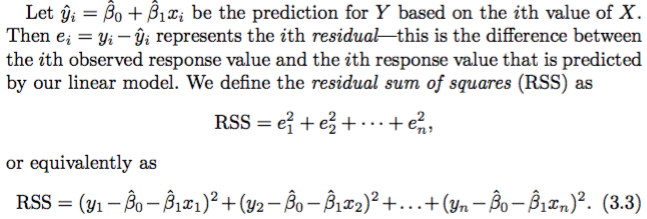
\includegraphics[width=8cm]{images/isl.png}
\end{figure}

ESL contains this excerpt on the second page of its linear regression section:

\begin{figure}[h]
\caption{Excerpt from ESL}
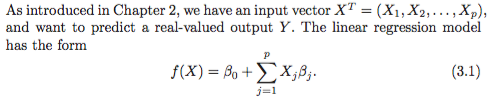
\includegraphics[width=8cm]{images/esl.png}
\end{figure}

While equations are necessary for describing the exact formulation of
regression, these textbooks place a significant emphasis on the theoretical
underpinnings of regression. Both ISL and ESL describe linear regression
mathematically for over 50 pages with over 30 equations (in the case of ESL,
84 equations) before giving their first exercise.

Simply based on way textbooks present the material, the learner can be misled
to believe that focusing on the mathematics of regression are the best way to
understand it when recent research in education suggests otherwise
\cite{van2010example}.

\subsection{Learning through online resources}

Another common approach to learn regression is through online resources. There
are a number of freely available articles and courses for the learner. However,
online content has high variability in its quality. For example, a Google
search of "intro to regression machine learning" yields several articles,
lecture slides, and links to Python libraries for machine learning.

This type of online content has a number of issues. In constrast to textbooks,
online articles have no promises of quality or completeness. Lecture slides are
usually posted without the accompanying lecture, making them difficult to
follow.

More glaringly, online articles typically contain very similar content to
textbooks. Most are primarily composed of text and images. While many online
articles are often easier for the layperson to understand, most do not help the
learner any more than textbooks do because the presentation of the content is
the same. A learner might as well go to a textbook to read about regression
since the content is presented more thoroughly.

\subsection{Learning in a traditional classroom setting}

Learning through a traditional classroom setting has a number of benefits over
textbook and online resource-based learning. For example, students are
encouraged to ask questions because they can receive immediate feedback. The
material is usually presented in a thorough way and asking the student to
complete assignments allows the student to actively engage with the material,
in stark contrast to the previous two learning methods.

However, the way students are evaluated in the classroom often creates
incentives that work against developing intuition for regression. Namely, the
majority of exams in these courses again place a large emphasis on the
mathematics of regression. In Stanford's CS229, all of their past exam problems
on regression involve heavy use of matrix algebra \cite{CS229:online}.
Most of their problems can be solved without prior knowledge of regression! A
student seeking to succeed on an exam in such a class would be incentivized to
understand calculus and linear algebra instead of regression.

\section{Approach}

All methods of learning have pros and cons. In this project, I choose to forgo
mathematical completeness and instead emphasize active learning. Whereas
textbooks, online articles, and lectures encourage passive learning through
absoption of information, I aim to encourage the learner to actively ask and
answer their own questions.

The basic premise of this project is to encourage the user to engage with the
concepts of regression through interaction and animation. For example, for the
introduction to linear regression the user can drag points around and see both
regression line and data immediately update. This naturally encourages the
follow questions:

\begin{enumerate}
  \item Does the slope become negative if the points curve downward?
  \item What if all the points lie on the same line except one point?
  \item What happens if all the points have the same x-value?
  \item What happens if all the points have the same y-value?
\end{enumerate}

The user can immediately test out these questions and get answers. Because of
this the user is encouraged to ask more questions, developing an understanding
of the behavior of regression through implicitly posing hypotheses. Then, the
user is equipped to connect their understanding with the mathematics. The
mathematics is a supplement to their intuition, not the other way around.

The rest of this section discusses the topics covered by this project and
typical questions that a user can pose and answer.

\subsection{Linear Regression}

In this section the project introduces the idea of linear regression as a
method of prediction. As mentioned earlier, the user is presented with a
scatterplot with the linear regression line overlain on top. The user can move
the points around and see the data, regression line, and regression equation
update in real-time. I then proceed to explain the least squares error
formulation. In addition to the questions mentioned above, this section allows
the user to answer the following questions:

\begin{enumerate}
  \item What is the squared error of a point when the line passes through the
  point?
  \item What is the error of a point when the line misses?
  \item Is the error larger when the line is further away from the point?
  \item Can the error have a negative value?
\end{enumerate}

\subsection{Polynomial Regression}

This section introduces polynomial regression as a way of dealing with
nonlinear patterns in the data. This section contains the same dataset with
multiple polynomials of increasing degrees overlain on top. When a point is
moved, all the curves update. This encourages the following questions:

\begin{enumerate}
  \item Can the degree 2 polynomial also fit a linear pattern?
  \item Can the degree 5 polynomial also fit a linear pattern?
  \item If the fitted degree 2 polynomial is concave down, is the degree 5
  polynomial also concave down?
\end{enumerate}

\subsection{Training Error}

This section introduces training error as a potenial method of evaluating
which regression model is the best fit for the data. This section allows the
user to move the data points, redrawing the regression curves and recalculating
the training error each time. This encourages the following questions:

\begin{enumerate}
  \item When does linear regression have lower training error than a degree 2
  polynomial?
  \item When does degree 2 polynomial have lower training error than a degree 5
  polynomial?
  \item Does a degree 5 polynomial always have a lower training error than a
  degree 2? Than a linear fit?
  \item Does a degree 10 polynomial always have a training error of 0 on this
  dataset?
\end{enumerate}

\subsection{Cross Validation}

This section explains why the training error is not an accurate way to select a
model and proceeds to explain why the cross validation error is more
appropriate. This section has little interactive parts because dragging
training set points makes the validation data invalid. However, it answers the
following questions:

\begin{enumerate}
  \item Does the validation error give a more accurate measure of model fit?
  \item If a model fits the training data perfectly, will it have a small
  validation error?
  \item If a model underfits the training data, will it also have a large
  validation error?
  \item Will increasing the degree of the polynomial always decrease the
  training error? The validation error?
\end{enumerate}

\section{Implementation}

This project is implemented as a web application. The code is open-source and
is available at \url{https://github.com/SamLau95/regression-explained}. The
majority of the code is written in ES6 Javascript, using the React
\cite{ReactAJa96:online} and Redux \cite{reactjsr26:online} libraries to render
the user interface and keep track of the application state. I used the
Highcharts \cite{Interact47:online} library to provide plotting functionality.

I used the publicly available dataset from Larry Winner (University of
Florida) on study on ice cream conducted in 1997 \cite{datasets42:online}
\cite{guinard1997sugar}.

\section{Results and Discussion}

The resulting web application is available at
\url{http://www.samlau.me/regression-explained/}. The page provides an
introduction to regression with interactive charts. Figures \ref{fig:app1} and
\ref{fig:app2} show the same chart before and after user interaction.

\begin{figure}[h]
\caption{Default dataset with fitted degree 5 polynomial}
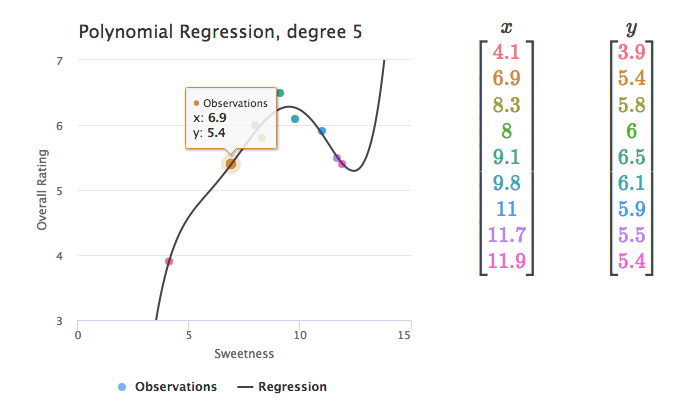
\includegraphics[width=8cm]{images/app1.png}
\label{fig:app1}
\end{figure}

\begin{figure}[h]
\caption{User-changed dataset with fitted degree 5 polynomial}
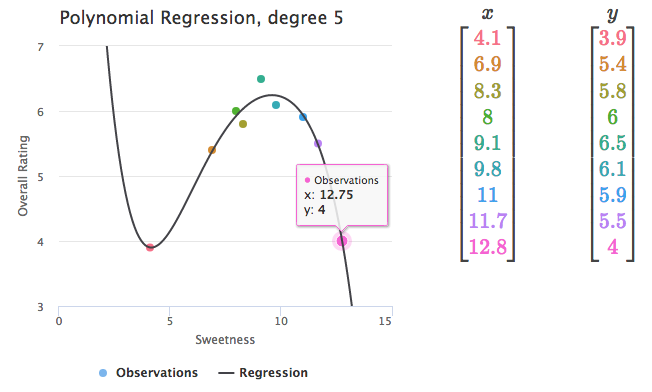
\includegraphics[width=8cm]{images/app2.png}
\label{fig:app2}
\end{figure}

I'm pleased with the result and the project has high user engagement among a
randomly selected beta test group (read: my friends). I hope that building this
project will help others develop an intuitive understanding for machine
learning through regression and I look forward to working on more educational
projects in the future.

\bibliographystyle{abbrv}
\bibliography{bibliography}

%\balancecolumns

\end{document}
